% experimental_setup.tex -- the experimental setup, on its own (the results are in
% presenting_results.tex). Hand-written: edit this file directly; build.py does not touch it.
% In Overleaf: Menu -> Main document -> experimental_setup.tex.
\documentclass[11pt]{article}
\usepackage[margin=1in]{geometry}
\usepackage[T1]{fontenc}
\usepackage{times}
\usepackage{amsmath}
\usepackage{amssymb}
\usepackage{booktabs}
\usepackage{graphicx}
\usepackage[hidelinks]{hyperref}
\usepackage{tikz}
\usetikzlibrary{positioning,arrows.meta,calc}
\usepackage{algorithm}
\usepackage{algpseudocode}
\usepackage{placeins}
\makeatletter
\setlength{\@fptop}{0pt}
\setlength{\@fpsep}{20pt}
\setlength{\@fpbot}{0pt plus 1fil}
\makeatother

\title{Seed-fate prediction: experimental setup}
\date{}
\begin{document}
\maketitle

\section{Experimental setup}
\begingroup
\setlength{\parskip}{0.8em plus 0.2em}
\setlength{\parindent}{0pt}

We group our experiments into two categories.

\subsection{Category 1: predicting the fate of a seed}

Given a trained diffusion model, we ask whether the outcome of sampling from a seed $x_T$, that
is, a sample from a particular mode or a hallucination, can be predicted without running the
sampler. We study this question on Gaussian mixtures, for which the true score is available in
closed form. Classifiers are fit on seeds whose outcome is computed with the true score, and are
evaluated on the outcomes produced by the learned model.

\paragraph{Setting.}
We consider deterministic samplers, which map a seed $x_T \sim \mathcal{N}(0, I)$ to a sample $x_0$
by integrating a probability-flow ODE driven by the score $\nabla_x \log p_t(x)$. We distinguish
the \emph{true score} of the data distribution from the \emph{learned score}, the neural
approximation used by the sampler.

\paragraph{Data.}
The data distribution is a mixture of $K$ isotropic Gaussians in $\mathbb{R}^d$,
\begin{equation}
    p(x) = \sum_{i=1}^{K} \pi_i \, \mathcal{N}(\mu_i, \sigma^2 I), \qquad \sigma = 0.1.
\end{equation}
Let $R_{99} = \sigma \sqrt{\chi^2_d(0.99)}$ denote the radius of the ball containing $99\%$ of the
mass of one component. The means are drawn on a sphere of radius $2\sqrt{d/2}$ with pairwise
distances of at least $3R_{99}$, so the balls are disjoint. We consider an \emph{unweighted}
mixture, $\pi_i = 1/K$, and a \emph{weighted} one, in which $K$ weights drawn from $U[0.3, 0.8]$
and normalised are assigned to the modes in a random order in each run. The two variants are
separate experiments with separately trained models.

\paragraph{Fate.}
The \emph{fate} of a seed $x_T$ is $k$ if its sample satisfies $\|x_0 - \mu_k\| \le R_{99}$, and
$-1$ (\emph{hallucination}) if $x_0$ lies outside every such ball. Fate prediction is therefore a
$(K + 1)$-class classification problem over the seed space.

\paragraph{Samplers.}
We consider two generative processes and three alternative solvers for one of them.

\textit{DDIM.} A variance-preserving diffusion,
$x_t = \sqrt{\bar\alpha_t}\, x_0 + \sqrt{1 - \bar\alpha_t}\, \epsilon$, with a linear schedule
$\beta_t \in [10^{-4}, 0.02]$ over 500 steps. The network is trained with the standard
$\epsilon$-prediction objective and sampled with the deterministic DDIM update, i.e.\ the Euler
discretisation of the probability-flow ODE (Song et al., 2021).

\textit{Flow matching.} The optimal-transport conditional path of Lipman et al.~(2023),
$x_t = (1 - (1 - \sigma_{\min})\,t)\, z + t\, x$ with $z \sim \mathcal{N}(0, I)$ and
$\sigma_{\min} = 10^{-4}$. The network regresses the conditional velocity and is sampled with 500
Euler steps. For uniformity we also denote its seed by $x_T$ and its sample by $x_0$.

\textit{Heun, RK45 and DPM-Solver++(2M).} The trained DDIM network, integrated on the same
500-step grid with a different solver: Heun's method (second order, 2 network evaluations per
step), fixed-step Dormand--Prince RK45 (fifth order, 6 evaluations per step) and DPM-Solver++(2M)
(Lu et al., 2022; second-order multistep, 1 evaluation per step). These samplers are not retrained.
They share the DDIM network and anchors and differ from DDIM only in the ground truth, which
isolates the effect of the discretisation.

\paragraph{Network.}
All learned models use the residual MLP of Figure~\ref{fig:scorenet}: four pre-LayerNorm residual
blocks with LeakyReLU(0.2) activations and a sinusoidal time embedding. The width is 256 for
$d \le 64$ and 1024 for $d \ge 128$. Models are trained with a mean-squared-error objective using
Adam and an exponential moving average of the weights (Table~\ref{tab:scorenet}). A model whose
hallucination rate on $10^4$ probe seeds exceeds $1.5\%$ is retrained once with $1.7\times$ the
number of steps.

\begin{figure}[htbp]
\centering
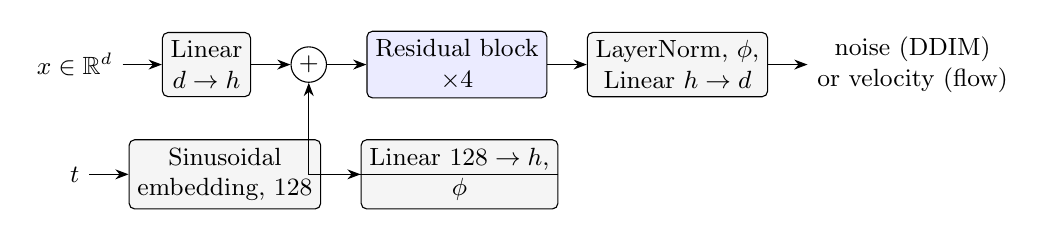
\begin{tikzpicture}[
    font=\small, >=Stealth, node distance=4mm and 5mm,
    blk/.style={draw, rounded corners=2pt, fill=gray!8, align=center, inner sep=3pt, minimum height=8mm},
    sum/.style={draw, circle, inner sep=0pt, minimum size=4.5mm}]
  \node (x) {$x \in \mathbb{R}^d$};
  \node[blk, right=of x] (lin) {Linear\\$d \to h$};
  \node[sum, right=of lin] (plus) {$+$};
  \node[blk, right=of plus, fill=blue!8] (res) {Residual block\\$\times 4$};
  \node[blk, right=of res] (head) {LayerNorm, $\phi$,\\Linear $h \to d$};
  \node[right=of head, align=center] (out) {noise (DDIM)\\or velocity (flow)};
  \node[below=9mm of x] (t) {$t$};
  \node[blk, right=of t] (emb) {Sinusoidal\\embedding, 128};
  \node[blk, right=of emb] (tm) {Linear $128 \to h$,\\$\phi$};
  \draw[->] (x) -- (lin);
  \draw[->] (lin) -- (plus);
  \draw[->] (plus) -- (res);
  \draw[->] (res) -- (head);
  \draw[->] (head) -- (out);
  \draw[->] (t) -- (emb);
  \draw[->] (emb) -- (tm);
  \draw[->] (tm.east) -| (plus.south);
\end{tikzpicture}

\vspace{5mm}
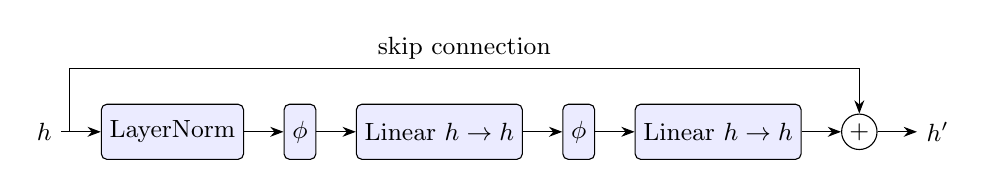
\begin{tikzpicture}[
    font=\small, >=Stealth, node distance=5mm,
    blk/.style={draw, rounded corners=2pt, fill=blue!8, align=center, inner sep=3pt, minimum height=7mm},
    sum/.style={draw, circle, inner sep=0pt, minimum size=4.5mm}]
  \node (in) {$h$};
  \node[blk, right=of in] (ln) {LayerNorm};
  \node[blk, right=of ln] (a1) {$\phi$};
  \node[blk, right=of a1] (w1) {Linear $h \to h$};
  \node[blk, right=of w1] (a2) {$\phi$};
  \node[blk, right=of a2] (w2) {Linear $h \to h$};
  \node[sum, right=of w2] (plus) {$+$};
  \node[right=of plus] (o) {$h'$};
  \draw[->] (in) -- (ln);
  \draw[->] (ln) -- (a1);
  \draw[->] (a1) -- (w1);
  \draw[->] (w1) -- (a2);
  \draw[->] (a2) -- (w2);
  \draw[->] (w2) -- (plus);
  \draw[->] (plus) -- (o);
  \draw[->] ($(in.east)+(1mm,0)$) -- ++(0,8mm) -| node[pos=0.25, above] {skip connection} (plus.north);
\end{tikzpicture}
\caption{\textbf{Score network.} Top: full network with hidden width $h$. Bottom: residual block.
$\phi$ denotes LeakyReLU(0.2).}
\label{fig:scorenet}
\end{figure}

\begin{table}[htbp]
\centering
\small
\caption{\textbf{Score network: architecture and training.}}
\label{tab:scorenet}
\begin{tabular}{ll}
\toprule
Hidden width                  & 256 for $d \le 64$; 1024 for $d \ge 128$ \\
Residual blocks               & 4 \\
Time embedding                & sinusoidal, dimension 128 \\
Activation                    & LeakyReLU(0.2) \\
Output                        & noise (DDIM) or velocity (flow matching) \\
\midrule
Training set                  & $10^5$ samples from $p$ \\
Optimiser                     & Adam, learning rate $10^{-3}$, cosine decay to $10^{-5}$ \\
Batch size                    & 512 \\
Gradient clipping             & norm 1 \\
Weight EMA                    & decay 0.999 \\
Training steps                & $30{,}000\,(1 + d/16)(1 + K/16)$ \\
Retraining                    & once, with $1.7\times$ the steps, if hallucination rate $> 1.5\%$ \\
Sampling steps                & 500 \\
\bottomrule
\end{tabular}
\end{table}

\paragraph{Anchors.}
The classifiers are trained on \emph{anchors}, seeds of known fate, obtained by integrating the
true-score probability-flow ODE backwards from labelled points in data space. For a budget of $b$
anchors per mode, we draw $b$ points uniformly in each $R_{99}$ ball (label $k$) and $b/2$ points
in the shell $R_{99} < \|x - \mu_k\| \le R_{99} + 2\sigma$ (label $-1$). Each point is written as
$x = \mu_k + \rho\, v$, with a direction $v = g / \|g\|$, $g \sim \mathcal{N}(0, I)$, which is
uniform on the unit sphere, and a radius $\rho$ drawn with $U \sim U[0, 1]$ as
\begin{equation}
    \rho = R_{99}\, U^{1/d} \quad \text{(ball)}, \qquad
    \rho = R_{99} + 2\sigma\, U \quad \text{(shell)}.
\end{equation}
The exponent $1/d$ makes the ball points uniform in volume. The shell points are uniform in
radius, which keeps them evenly spread across the band in high dimension, where a
volume-uniform draw would concentrate them at its outer edge. These points are then mapped to the
seed space by running the sampler backwards with the true score, in $T$ steps
(Figure~\ref{fig:pipeline}, top). For DDIM, each backward step is a DDIM update whose noise
prediction is the average of the exact $\epsilon$ at both ends of the step, a Heun-type
correction that makes the map second order; the learned DDIM sampler itself uses the plain,
first-order update. For flow matching, the exact velocity field is integrated backwards with
Heun's method. The shell points provide hallucination labels adjacent to the
mode boundaries.

\paragraph{Ground truth.}
The test set consists of $50{,}000 \cdot K$ seeds $x_T \sim \mathcal{N}(0, I)$, labelled by their
fate under the learned sampler (Figure~\ref{fig:pipeline}, bottom). The classifiers never query the
learned model, so the evaluation measures how well true-score anchors predict its behaviour. The
number of backward steps $T$ affects only the anchors.

\begin{figure}[htbp]
\centering
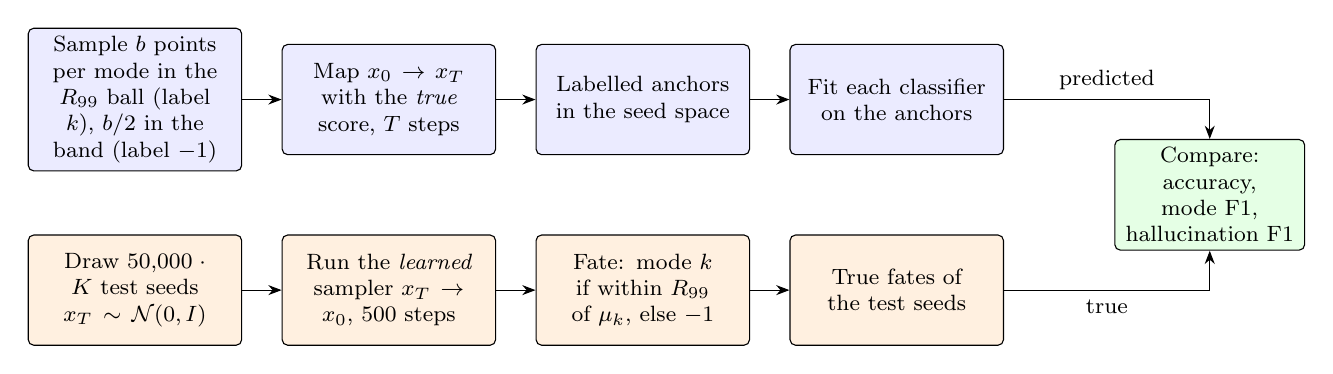
\begin{tikzpicture}[
    font=\footnotesize, >=Stealth, node distance=4mm and 5mm,
    blk/.style={draw, rounded corners=2pt, align=center, text width=25mm, inner sep=3pt, minimum height=14mm},
    top/.style={blk, fill=blue!8}, bot/.style={blk, fill=orange!12},
    res/.style={blk, fill=green!10, text width=22mm}]
  \node[top] (a1) {Sample $b$ points per mode in the $R_{99}$ ball (label $k$), $b/2$ in the band (label $-1$)};
  \node[top, right=of a1] (a2) {Map $x_0 \to x_T$ with the \emph{true} score, $T$ steps};
  \node[top, right=of a2] (a3) {Labelled anchors in the seed space};
  \node[top, right=of a3] (a4) {Fit each classifier on the anchors};
  \node[bot, below=8mm of a1] (g1) {Draw $50{,}000 \cdot K$ test seeds $x_T \sim \mathcal{N}(0, I)$};
  \node[bot, right=of g1] (g2) {Run the \emph{learned} sampler $x_T \to x_0$, 500 steps};
  \node[bot, right=of g2] (g3) {Fate: mode $k$ if within $R_{99}$ of $\mu_k$, else $-1$};
  \node[bot, right=of g3] (g4) {True fates of the test seeds};
  \node[res, right=14mm of $(a4.east)!0.5!(g4.east)$] (m) {Compare:\\accuracy,\\mode F1,\\hallucination F1};
  \draw[->] (a1) -- (a2);
  \draw[->] (a2) -- (a3);
  \draw[->] (a3) -- (a4);
  \draw[->] (g1) -- (g2);
  \draw[->] (g2) -- (g3);
  \draw[->] (g3) -- (g4);
  \draw[->] (a4.east) -| node[pos=0.25, above] {predicted} (m.north);
  \draw[->] (g4.east) -| node[pos=0.25, below] {true} (m.south);
\end{tikzpicture}
\caption{\textbf{Evaluation protocol.} Top: anchors are placed around each mode and mapped to the
seed space with the true score; the classifiers are fit on them. Bottom: test seeds are labelled
by the learned sampler. The classifiers are evaluated on the same test seeds.}
\label{fig:pipeline}
\end{figure}

\paragraph{Metrics.}
We report overall accuracy over the $K + 1$ classes, the F1 score macro-averaged over the $K$ mode
classes, and the F1 score of the hallucination class. Since hallucinations are rare, accuracy is
dominated by mode seeds, and hallucination F1 is the relevant measure of detection. All results
are means over three runs, each with independent means, network initialisation and test seeds.

\paragraph{Classifiers.}
We compare four classifiers, configured as in Table~\ref{tab:fatenets}.

\textit{kNN.} Majority vote among the $k = 10$ nearest anchors in Euclidean distance.

\textit{Altered kNN.} Trained on mode anchors only, it detects hallucinations as seeds whose
neighbourhood has inconsistent labels. Around each mean, $b/5$ points are placed on each of five
spheres of radius $0.3jR_{99}$, $j = 1, \dots, 5$ (with $\rho = 0.3jR_{99}$ and $v$ as above), weighted linearly in the radius from $0.84$ to
$0.2$, and mapped back as above. Given the weights $w_j$ and labels $y_j$ of the 10 nearest anchors,
\begin{equation}
    s_c = \frac{\sum_j w_j \, \mathbf{1}[y_j = c]}{\sum_j w_j}, \qquad
    p = \mathrm{softmax}(s / \tau), \quad \tau = 0.1.
\end{equation}
A seed is classified as a hallucination if $1 - H(p)/\log K < \theta$, where $H$ is the Shannon
entropy, and as $\arg\max_c p_c$ otherwise. The threshold $\theta$ maximises hallucination F1 on
5{,}000 held-out seeds labelled with the true score, over 100 candidates spanning the
$0.5\%$--$50\%$ quantiles of the confidence.

\textit{Quadratic network.} Multinomial logistic regression on the features $x_i$ and
$x_i x_j$ ($i \le j$), which yields quadratic decision boundaries.

\textit{Polar network.} Motivated by the concentration of $\|x_T\|$ around $\sqrt{d}$, it
parametrises a seed by its direction $u = x / \|x\|$ and radial offset $r = \|x\| - \sqrt{d}$.
A linear map gives $z \in \mathbb{R}^{256}$ from $(u, r)$, and the mode logits are linear in
$(z, z^2, z^3)$, with element-wise powers. The hallucination logit is
\begin{equation}
    \ell_{\text{hall}} = c + a\,r - b\,(\ell_1 - \ell_2), \qquad b > 0,
\end{equation}
where $\ell_1 \ge \ell_2$ are the two largest mode logits. Hallucinations are thus predicted near
the boundary between the two most likely modes, with a margin that depends on the radius.

The quadratic and polar networks are trained with cross-entropy over the $K + 1$ classes on all
anchors, as ensembles of three models whose log-probabilities are summed.

\begin{table}[htbp]
\centering
\small
\caption{\textbf{Classifier settings.}}
\label{tab:fatenets}
\begin{tabular}{lll}
\toprule
Classifier & Setting & Value \\
\midrule
kNN            & neighbours                    & 10 \\
\midrule
Altered kNN    & neighbours                    & 10 \\
               & spheres per mode              & 5, radius $0.3R_{99}$ to $1.5R_{99}$ \\
               & anchor weights                & 0.84 to 0.2, linear in the radius \\
               & softmax temperature           & 0.1 \\
               & threshold $\theta$            & best hallucination F1 on 5{,}000 seeds \\
\midrule
Quadratic      & features                      & $x_i$ and $x_i x_j$, $i \le j$ \\
\midrule
Polar          & hidden size, degree           & 256, 3 \\
\midrule
Quadratic and  & optimiser                     & AdamW, learning rate $3 \times 10^{-3}$, one-cycle \\
polar          & weight decay, batch size      & $10^{-4}$, 2{,}048 \\
               & epochs                        & 30 (at least 3{,}000 steps) \\
               & ensemble                      & 3 models \\
\bottomrule
\end{tabular}
\end{table}

\paragraph{The experiment.}
An experiment is specified by the sampler, the mixture variant, $K$, $d$, the number of backward
steps $T$ and the anchor budget $b$. Algorithm~\ref{alg:protocol} summarises the procedure for one
configuration. Lines 2--4 depend on neither $T$ nor $b$, so the trained model and the test set are
shared across both. We evaluate every combination in Table~\ref{tab:grid}; each is one entry of the
result tables that follow.

\begin{algorithm}[htbp]
\caption{Evaluation protocol for one configuration (sampler, mixture variant, $K$, $d$, $T$, $b$)}
\label{alg:protocol}
\begin{algorithmic}[1]
\For{run $= 1, 2, 3$}
  \State Draw the means $\mu_i$ (and, if weighted, the weights $\pi_i$).
  \State Train the score network; retrain once if it hallucinates on $> 1.5\%$ of seeds.
  \State \textbf{Ground truth:} fates of $50{,}000 \cdot K$ seeds $x_T \sim \mathcal{N}(0, I)$ under the learned sampler.
  \State \textbf{Anchors:} $b$ points per mode in the ball, $b/2$ in the band; map back with the true score.
  \For{each classifier}
    \State Fit it on the anchors (altered kNN: ring anchors, $\theta$ from 5{,}000 seeds).
    \State Predict the fates of the test seeds; compute accuracy, mode F1, hallucination F1.
  \EndFor
\EndFor
\State \Return each metric averaged over the three runs.
\end{algorithmic}
\end{algorithm}

\begin{table}[htbp]
\centering
\small
\caption{\textbf{Experiment grid.}}
\label{tab:grid}
\begin{tabular}{ll}
\toprule
Sampler                         & DDIM, flow matching; Heun, RK45, DPM-Solver++(2M) (DDIM network) \\
Mixing weights                  & uniform; random (drawn from $U[0.3, 0.8]$, normalised) \\
Number of modes $K$             & 2, 4, 8, 16 \\
Dimension $d$                   & 2, 4, 8, 16, 32, 64, 128, 256 ($K = 16$, $d = 2$ not run) \\
True-score steps $T$            & 250, 500, 750 \\
Anchors per mode $b$            & 2{,}000, 5{,}000, 10{,}000, 15{,}000, 20{,}000 \\
Test seeds                      & $50{,}000 \cdot K$ (100{,}000 to 800{,}000) \\
Calibration seeds               & 5{,}000 (altered kNN only) \\
Runs                            & 3 \\
\bottomrule
\end{tabular}
\end{table}

\FloatBarrier
\subsection{Category 2: seed fates in image latent spaces}

Category~1 relies on a data distribution that is exactly a Gaussian mixture. We now ask whether
fate prediction carries over to real data, whose distribution is only approximately a mixture. We
train an autoencoder whose latent space is shaped to resemble the mixtures of Category~1, run a
latent diffusion model in that space, and predict the fate of its seeds as before.

\paragraph{Setting.}
The setting is that of Category~1, with the synthetic mixture replaced by the latent space of an
image autoencoder. Since this space has no exact mixture density, the true score is that of a
mixture fitted to the latents, and the learned score is trained on the latents themselves.

\paragraph{Data.}
We use MNIST, Fashion-MNIST and CIFAR-10, each with its $K = 10$ classes, and a latent dimension
of $d = 32$. For each dataset we train a convolutional autoencoder with encoder $E$ and decoder
$G$. The encoder sees only images, but the loss uses class labels to impose the geometry of
Category~1 on the latents $z = E(x)$:
\begin{equation}
\begin{aligned}
    \mathcal{L} = \; & \|x - G(z + \xi)\|^2
    + \lambda_{\text{sep}}\, \mathbb{E}_{y_i \ne y_j} \max\!\Bigl(0, \tfrac{D - \|z_i - z_j\|}{\sigma}\Bigr)^{2} \\
    & + \frac{\lambda_{\text{cov}}}{K} \sum_{c} \Bigl\| \tfrac{\mathrm{Cov}_c(z)}{\sigma^2} - I \Bigr\|_F^2
    + \frac{\lambda_{\text{norm}}}{K} \sum_{c} \max\!\Bigl(0, \tfrac{\|m_c\| - R}{\sigma}\Bigr)^{2},
\end{aligned}
\end{equation}
where $\xi \sim \mathcal{N}(0, (0.15\,\sigma)^2 I)$, $\mathrm{Cov}_c$ and $m_c$ are the latent
covariance and mean of class $c$, and $\lambda_{\text{sep}} = 5$, $\lambda_{\text{cov}} = 2$ and
$\lambda_{\text{norm}} = 1$. The constants are those of Category~1: $\sigma = 0.1$,
$R = 2\sqrt{d/2}$ and $D = 3R_{99}$. The terms ask for latents of different classes to be at least
$D$ apart, for each class to have covariance $\sigma^2 I$, and for the class means to lie within
radius $R$; the means themselves are not prescribed. Fashion-MNIST and CIFAR-10 are trained with
random flips and shifts, so that test images also fall inside their clusters.

The resulting latent distribution is only approximately Gaussian. We therefore fit a mixture to
the encoded training set without labels: $k$-means with $K = 10$ gives the means $\hat\mu_i$, the
relative cluster sizes give the weights $\hat\pi_i$, and the pooled within-cluster variance gives
$\hat\sigma^2$. $R_{99}$ is computed per cluster, and the largest value is used throughout. Labels
are used only afterwards, to name each cluster by its majority class.

\paragraph{Fate.}
As in Category~1, with one change: because the latents do not fill the fitted balls exactly, the
radius is enlarged. The fate of a seed is $k$ if its sample satisfies
$\|x_0 - \hat\mu_k\| \le 1.25\,R_{99}$, and $-1$ otherwise.

\paragraph{Samplers.}
We use DDIM only, with the schedule of Category~1 over 200 steps.

\paragraph{Network.}
The score network is that of Figure~\ref{fig:scorenet}, with width 256, trained on the encoded
training images rather than on samples of the fitted mixture. We deliberately train it for a
tenth of the Category~1 budget, $3{,}000\,(1 + d/16)(1 + K/16)$ steps, without retraining: a fully
trained model hallucinates on about $0.3\%$ of seeds, too few to evaluate detection. The
hallucinations of this model are mostly near misses, whose samples land just outside a ball.

\paragraph{Anchors.}
Anchors are sampled as in Category~1, with $b$ points in each ball of radius $1.25\,R_{99}$ and
$b/2$ in the surrounding shell of width $2\hat\sigma$. Unlike Category~1, they are mapped to the
seed space by inverting the \emph{learned} DDIM sampler, with two fixed-point iterations per step,
so that sampling from an anchor seed returns the anchor exactly. The anchors therefore describe
the learned model directly.

\paragraph{Ground truth.}
The test set consists of $100{,}000$ seeds $x_T \sim \mathcal{N}(0, I)$, labelled by their fate
under the learned sampler.

\paragraph{Metrics.}
The three metrics of Category~1. We add one baseline, the \emph{true score}: each test seed is
mapped forward with the exact score of the fitted mixture, and its fate is compared with that under
the learned sampler. This measures how well the fitted mixture alone predicts the learned model,
without anchors or a classifier. As an independent check, a CNN classifier trained on each dataset
reads the decoded samples, to verify that a sample inside ball $k$ decodes to an image of the
class of cluster $k$.

\paragraph{Classifiers.}
The four classifiers of Category~1, with the settings of Table~\ref{tab:fatenets}. The
altered-kNN threshold is calibrated on 5{,}000 seeds labelled by the learned sampler, consistent
with the anchors.

\paragraph{The experiment.}
An experiment is specified by the dataset and the anchor budget $b$. Algorithm~\ref{alg:protocol2}
summarises the procedure, and Table~\ref{tab:grid2} lists the settings.

\begin{algorithm}[!htbp]
\caption{Evaluation protocol for Category 2, for one dataset and anchor budget $b$}
\label{alg:protocol2}
\begin{algorithmic}[1]
\For{run $= 1, 2, 3$}
  \State Train the autoencoder; encode the training set.
  \State Fit a 10-component mixture to the latents with $k$-means (no labels).
  \State Train the DDIM score network on the latents (reduced budget).
  \State \textbf{Ground truth:} fates of $100{,}000$ seeds under the learned sampler.
  \State \textbf{Baseline:} fates of the same seeds under the fitted mixture's exact score.
  \State \textbf{Anchors:} $b$ points per ball, $b/2$ in the shell; invert the learned sampler.
  \For{each classifier}
    \State Fit it on the anchors; predict the test fates; compute the three metrics.
  \EndFor
\EndFor
\State \Return each metric averaged over the three runs.
\end{algorithmic}
\end{algorithm}

\begin{table}[!htbp]
\centering
\small
\caption{\textbf{Category 2 settings.}}
\label{tab:grid2}
\begin{tabular}{ll}
\toprule
Datasets                        & MNIST, Fashion-MNIST, CIFAR-10 ($K = 10$ classes each) \\
Latent dimension $d$            & 32 \\
Autoencoder                     & convolutional; 300 epochs; flips and shifts for Fashion-MNIST, CIFAR-10 \\
Fitted mixture                  & $k$-means, $K = 10$; pooled $\hat\sigma$; weights from cluster sizes \\
Fate radius                     & $1.25\,R_{99}$ \\
Sampler                         & DDIM, 200 steps \\
Score-network training          & $3{,}000\,(1 + d/16)(1 + K/16)$ steps, no retraining \\
Anchor mapping                  & inversion of the learned sampler \\
Anchors per mode $b$            & 10{,}000, 50{,}000, 100{,}000 \\
Test seeds                      & 100{,}000 \\
Calibration seeds               & 5{,}000, labelled by the learned sampler \\
Runs                            & 3 \\
\bottomrule
\end{tabular}
\end{table}

\FloatBarrier
\subsection{How the visualisations are generated}

Every table and heatmap is drawn from the saved results of the runs; nothing is recomputed. The
animations are produced separately from the trained models. The same conventions hold
throughout: a hallucination is drawn as a red cross, the modes in colours that never include red,
and the solid circle around a mode is its $R_{99}$ ball.

\paragraph{Category 1: result tables.}
One table per sampler, mixture variant and anchor budget $b$.
\begin{enumerate}
    \item For every configuration of Table~\ref{tab:grid}, Algorithm~\ref{alg:protocol} gives the
    overall accuracy of each classifier, averaged over the three runs.
    \item Each row of a table is one $(K, d)$ pair. Each classifier has three sub-columns, the
    number of true-score steps $T = 250, 500, 750$ used to build the anchors.
    \item Within a row, the best classifier at each $T$ is set in bold. The configuration $K = 16$,
    $d = 2$ was not run and is shown as --.
\end{enumerate}

\paragraph{Category 1: heatmaps.}
One figure per sampler, mixture variant, $T$ and anchor budget $b$.
\begin{enumerate}
    \item The figure is a grid of panels: one row per classifier (kNN, altered kNN, quadratic,
    polar) and one column per metric (overall accuracy, mode F1, hallucination F1).
    \item Within a panel, the vertical axis is the number of modes $K \in \{2, 4, 8, 16\}$ and the
    horizontal axis the dimension $d \in \{2, \dots, 256\}$. Each cell holds the metric in percent,
    averaged over the three runs, printed in the cell and coloured on a fixed 0--100 scale, so that
    all heatmaps are directly comparable. Empty cells were not run.
\end{enumerate}

\paragraph{Category 1: two-dimensional animations.}
To show what the classifiers have to learn, we animate the case $d = 2$, $K = 4$ with the models of
the first run, for every sampler and both mixture variants. There are three animations.

\textit{(a) Learned score: where hallucinations come from.}
\begin{enumerate}
    \item Draw $80{,}000$ seeds $x_T \sim \mathcal{N}(0, I)$.
    \item Run the learned sampler (500 steps) and record the position of every seed every 5 steps.
    For Heun, RK45 and DPM-Solver++(2M), the positions are those of the solver's own steps.
    \item Label each seed by the fate of its sample $x_0$.
    \item Keep every hallucinating seed (about $1.2\%$, i.e.\ roughly 950) and 4{,}000 of the other
    seeds at random. Hallucinations are rare, so with fewer seeds too few of them would remain to
    show the boundaries. The title of each animation states both counts and the true rate.
    \item Play the recorded paths backwards, from the samples $x_0$ to the seeds $x_T$ they came
    from. The left panel shows the samples in data space; on the right the points move, keeping the
    colour of their fate. The view zooms out from the modes to the seed space, and the $R_{99}$
    circles fade as the points leave data space. A counter gives the step, with 0 the generated
    sample $x_0$ and 499 the seed $x_T$.
\end{enumerate}
In the last frame, the hallucinating seeds lie on thin curves between the regions of seeds that
reach each mode, and far out in the tails of $\mathcal{N}(0, I)$.

\textit{(b) True score.} The same as (a), with the true score in place of the learned one (DDIM
and flow matching only; Heun, RK45 and DPM-Solver++(2M) share the DDIM true score).

\textit{(c) Anchors.}
\begin{enumerate}
    \item Draw the anchors exactly as in the \emph{Anchors} paragraph, for the best budget of this
    case: $b = 20{,}000$ per mode, with which kNN reaches $98.9\%$ overall accuracy.
    \item Show 400 random anchors per ball and 200 per shell. The path of each anchor does not
    depend on the others, so the paths shown are exactly those of the full set.
    \item Map the anchors from data space to the seed space with the true score in 500 steps,
    recording every 5 steps. The left panel shows the anchors where they are placed; the shell is
    shaded red, with a dashed outer edge. On the right the anchors move to their seeds.
\end{enumerate}
In the last frame, the shell anchors lie on the same curves as the hallucinating seeds of (a).
This is why anchors, which never query the learned model, can predict its hallucinations.

\paragraph{Category 2: result tables and heatmaps.}
These are built as in Category 1, with the dataset in place of the number of modes: each row of a
table is a dataset (MNIST, Fashion-MNIST, CIFAR-10, $K = 10$), and each heatmap panel is
datasets $\times$ latent dimension.

\paragraph{Category 2: decoded samples.}
These show what the seed regions predicted by each classifier look like as images. For each
dataset, run and classifier:
\begin{enumerate}
    \item Draw $10{,}000$ fresh seeds $x_T \sim \mathcal{N}(0, I)$.
    \item Fit the classifier on the anchors as in Algorithm~\ref{alg:protocol2}, at the largest
    anchor budget, and predict the class of every seed: one of the 10 clusters, or hallucination.
    \item For each predicted class, take the first 10 seeds whose learned sample clearly belongs to
    it, run the learned sampler and decode the sample with $G$. A cluster's images must land within
    $0.7\,R_{99}$ of its centre, and a hallucination's beyond $1.25\,R_{99}$ from every centre; this
    is stricter than the fate rule, so the grids show unambiguous cases.
    \item Arrange one row per class: the decoded cluster mean, then the 10 images. A row for a
    cluster shows images of its majority class. The hallucination row shows decoded samples that
    fall between clusters.
\end{enumerate}

\paragraph{Category 2: hallucination check.}
For all $10{,}000$ seeds, we know where the learned sampler actually sends them. For each
classifier we therefore report:
\begin{itemize}
    \item the precision of its hallucination flags (the fraction of flagged seeds that really
    hallucinate), compared with the base rate of a random seed;
    \item its recall;
    \item the distance of the flagged samples to their nearest cluster centre, in units of $R_{99}$;
    \item the confidence of the dataset's CNN classifier on their decoded images;
    \item the flagged images themselves, each marked H (really hallucinates) or M (lands in a cluster).
\end{itemize}
A single panel places the precision and recall of all classifiers side by side.

\endgroup

\end{document}
